% Compile with XeLaTeX or LuaLaTeX
\documentclass[12pt,a4paper]{article}

\usepackage[a4paper,margin=2.5cm]{geometry}
\usepackage{fontspec}
\usepackage{polyglossia}
\setmainlanguage{greek}
\setotherlanguage{english}
\setmainfont{DejaVu Serif}
\setsansfont{DejaVu Sans}
\setmonofont{DejaVu Sans Mono}
\newfontfamily\greekfont[Script=Greek]{DejaVu Serif}
\newfontfamily\greekfontsf[Script=Greek]{DejaVu Sans}
\newfontfamily\greekfonttt[Script=Greek]{DejaVu Sans Mono}
\usepackage{graphicx}
\usepackage{array}
\usepackage{booktabs}
\usepackage{tabularx}
\usepackage{float}
\usepackage{amsmath}
\usepackage{hyperref}
\usepackage{caption}
\usepackage{pdflscape}
\usepackage{fancyhdr}

\hypersetup{
  colorlinks=true,
  linkcolor=black,
  urlcolor=blue
}

\pagestyle{fancy}
\fancyhf{}
\fancyfoot[C]{\thepage}
\renewcommand{\headrulewidth}{0pt}
\renewcommand{\footrulewidth}{0pt}
\fancypagestyle{plain}{
  \fancyhf{}
  \fancyfoot[C]{\thepage}
  \renewcommand{\headrulewidth}{0pt}
  \renewcommand{\footrulewidth}{0pt}
}

\setlength{\parindent}{0pt}
\setlength{\parskip}{0.65em}
\renewcommand{\arraystretch}{1.2}

\newcolumntype{L}{>{\raggedright\arraybackslash}X}
\newcolumntype{C}[1]{>{\centering\arraybackslash}p{#1}}

\begin{document}

\begin{titlepage}
\centering

{\Large Αριστοτέλειο Πανεπιστήμιο Θεσσαλονίκης\par}
{\large Τμήμα Μηχανολόγων Μηχανικών\par}
\vspace{1.8cm}

{\LARGE\bfseries Υπολογισμός Ψυκτικού Φορτίου Κατοικίας\par}
\vspace{0.5cm}
{\Large Report για τα υποερωτήματα α και β της εργασίας\par}
\vspace{0.8cm}
{\large Κτίριο Γ1 -- Κάτοψη Ισογείου\par}
\vspace{1.6cm}

\begin{tabular}{>{\bfseries}p{4.2cm}p{9.2cm}}
Μάθημα: & Κλιματισμός \\
Θέμα: & Τεκμηρίωση κτιρίου, συμβολισμών και θερμοφυσικών δεδομένων \\
Τοποθεσία έργου: & Θεσσαλονίκη \\
Κλιματική ζώνη: & Ζώνη Γ' κατά Κ.Εν.Α.Κ. \\
\end{tabular}

\vfill
{\large \today\par}
\thispagestyle{fancy}
\end{titlepage}

\tableofcontents
\newpage

\section{Εισαγωγή / Σκοπός}

Η παρούσα εργασία εντάσσεται στο πλαίσιο του μαθήματος του Κλιματισμού και έχει ως
γενικό αντικείμενο τον υπολογισμό των ψυκτικών φορτίων κατοικίας και τη διαμόρφωση
των βασικών παραμέτρων του συστήματος κλιματισμού. Για να είναι δυνατός ο τελικός
υπολογισμός των φορτίων, είναι απαραίτητο να προηγηθεί μία συστηματική τεκμηρίωση
του κτιρίου προς μελέτη, της γεωμετρίας του, του εξωτερικού περιβλήματος, των
ανοιγμάτων και των θερμοφυσικών χαρακτηριστικών των δομικών στοιχείων.

Το τελικό report της εργασίας θα οργανωθεί σε οκτώ βασικές ενότητες. Στο παρόν
στάδιο αναπτύσσονται οι τέσσερις πρώτες:

\begin{itemize}
\item η εισαγωγή και ο σκοπός της εργασίας,
\item ο πίνακας βασικών συμβόλων,
\item και η αναλυτική παρουσίαση του κτιρίου προς μελέτη.
\item ο αναλυτικός υπολογισμός των ψυκτικών φορτίων με τη μέθοδο CLTD της ASHRAE.
\end{itemize}

Συνεπώς, ο βασικός στόχος του παρόντος κειμένου είναι να διαμορφώσει με ακρίβεια και
με ενιαία τεχνική ορολογία τη βάση δεδομένων πάνω στην οποία θα στηριχθούν τα επόμενα
στάδια της μελέτης, δηλαδή:

\begin{itemize}
\item ο υπολογισμός των αισθητών και λανθανόντων ψυκτικών φορτίων,
\item η επιλογή και διαστασιολόγηση του συστήματος κλιματισμού,
\item και η μελέτη των υποσυστημάτων ανάκτησης και νερού.
\end{itemize}

\subsection{Αντικείμενο της παρούσας φάσης}

Στην τρέχουσα φάση η εργασία επικεντρώνεται στην τεκμηρίωση του \textbf{Κτιρίου Γ1},
δηλαδή της κάτοψης ισογείου κατοικίας που θα αποτελέσει τη θερμική ζώνη αναφοράς.
Ειδικότερα, προσδιορίζονται:

\begin{itemize}
\item οι συνολικές διαστάσεις και το εμβαδόν της κάτοψης,
\item οι επιμέρους λειτουργικοί χώροι,
\item ο προσανατολισμός των όψεων,
\item τα ανοίγματα ανά όψη,
\item οι ακαθάριστες και καθαρές επιφάνειες των εξωτερικών τοίχων,
\item οι συντελεστές θερμοπερατότητας \(U\) των βασικών δομικών στοιχείων,
\item και ο μέσος συντελεστής θερμοπερατότητας \(U_m\) του προς μελέτη κελύφους.
\end{itemize}

\subsection{Βασική μεθοδολογική παραδοχή}

Αν και η αρχιτεκτονική κάτοψη περιλαμβάνει περισσότερους του ενός χώρους
(καθιστικό, τραπεζαρία, κουζίνα, WC και χώλ), για τους θερμικούς υπολογισμούς το
ισόγειο θα αντιμετωπιστεί ως \textbf{μία ενιαία θερμική ζώνη}. Αυτό σημαίνει ότι τα
εσωτερικά χωρίσματα δεν θεωρούνται στοιχεία με ουσιώδη θερμική ροή μεταξύ χώρων με
διαφορετικές συνθήκες λειτουργίας, αλλά εσωτερικοί διαχωρισμοί του ίδιου
κλιματιζόμενου όγκου. Η παραδοχή αυτή δεν αναιρεί τη σημασία της αρχιτεκτονικής
διαρρύθμισης, η οποία εξακολουθεί να είναι απαραίτητη για τον εντοπισμό των
ανοιγμάτων, των εκτεθειμένων δομικών στοιχείων και της χρήσης κάθε τμήματος του
κτιρίου.

\section{Πίνακας βασικών συμβόλων}

\subsection{Γενικά σύμβολα και θερμικά μεγέθη}

\begin{table}[H]
\centering
\small
\caption{Βασικά σύμβολα που χρησιμοποιούνται στα Sections 1--4}
\begin{tabularx}{\textwidth}{C{2.2cm} L C{2.8cm}}
\toprule
\textbf{Σύμβολο} & \textbf{Περιγραφή} & \textbf{Μονάδα} \\
\midrule
\(A\) & Επιφάνεια δομικού στοιχείου ή ανοίγματος & \(\mathrm{m^2}\) \\
\(A_{\text{ακ.}}\) & Ακαθάριστη επιφάνεια τοίχου πριν από την αφαίρεση ανοιγμάτων & \(\mathrm{m^2}\) \\
\(A_{\text{καθ.}}\) & Καθαρή επιφάνεια τοίχου μετά την αφαίρεση ανοιγμάτων & \(\mathrm{m^2}\) \\
\(A_{\text{ανοιγμ.}}\) & Επιφάνεια ανοίγματος ή συνολική επιφάνεια ανοιγμάτων & \(\mathrm{m^2}\) \\
\(U\) & Συντελεστής θερμοπερατότητας συγκεκριμένου δομικού στοιχείου & \(\mathrm{W/(m^2K)}\) \\
\(U_m\) & Μέσος συντελεστής θερμοπερατότητας του εξεταζόμενου κελύφους & \(\mathrm{W/(m^2K)}\) \\
\(L\) & Μήκος δομικού στοιχείου ή πλευράς κάτοψης & \(\mathrm{m}\) \\
\(H\) & Ύψος ορόφου & \(\mathrm{m}\) \\
\(P\) & Περίμετρος κάτοψης & \(\mathrm{m}\) \\
\midrule
\(A_{\text{δαπ.}}\) & Εμβαδόν δαπέδου ισογείου & \(\mathrm{m^2}\) \\
\(A_{\text{οροφ.}}\) & Εμβαδόν οροφής σε επαφή με εξωτερικό αέρα & \(\mathrm{m^2}\) \\
\(A_{\text{τοίχων}}\) & Συνολικό εμβαδόν εξωτερικών τοίχων & \(\mathrm{m^2}\) \\
\bottomrule
\end{tabularx}
\end{table}

\subsection{Συμβολισμοί δομικών στοιχείων του κτιρίου}

Για τη συστηματική παρουσίαση του κτιρίου και την ομοιόμορφη αναφορά σε όλα τα επόμενα
βήματα της εργασίας, χρησιμοποιείται ένας απλός και συνεπής συμβολισμός για τα
δομικά στοιχεία του εξωτερικού περιβλήματος.

\begin{table}[H]
\centering
\small
\caption{Συμβολισμοί αδιαφανών και διαφανών στοιχείων}
\begin{tabularx}{\textwidth}{C{2.6cm} L}
\toprule
\textbf{Συμβολισμός} & \textbf{Ερμηνεία} \\
\midrule
\(W_{L\mathrm{B}}\) & Εξωτερικός αδιαφανής τοίχος βόρειας όψης \\
\(W_{L\mathrm{N}}\) & Εξωτερικός αδιαφανής τοίχος νότιας όψης \\
\(W_{L\mathrm{A}}\) & Εξωτερικός αδιαφανής τοίχος ανατολικής όψης \\
\(W_{L\Delta}\) & Εξωτερικός αδιαφανής τοίχος δυτικής όψης \\
\(R\) & Οροφή σε επαφή με εξωτερικό αέρα \\
\(F\) & Δάπεδο σε επαφή με το έδαφος \\
\(W_{i\mathrm{B}1}\) & Πρώτο παράθυρο βόρειας όψης \\
\(W_{i\mathrm{B}2}\) & Δεύτερο παράθυρο βόρειας όψης \\
\(W_{i\mathrm{N}}\) & Παράθυρο νότιας όψης \\
\(W_{i\mathrm{A}}\) & Μπαλκονόπορτα ανατολικής όψης \\
\(W_{i\Delta}\) & Μπαλκονόπορτα δυτικής όψης \\
\bottomrule
\end{tabularx}
\end{table}

\section{Κτίριο προς μελέτη}

\subsection{Σύντομη περιγραφή του κτιρίου}

Το εξεταζόμενο κτίριο είναι το \textbf{Κτίριο Γ1}, δηλαδή ισόγεια κατοικία ορθογωνικής
κάτοψης με εξωτερικές διαστάσεις \(10.00\,\mathrm{m} \times 14.50\,\mathrm{m}\).
Το συνολικό εμβαδόν του ισογείου ισούται με:

\[
A_{\text{δαπ.}} = 10.00 \times 14.50 = 145.00\,\mathrm{m^2}
\]

Το ύψος του ορόφου θεωρείται:

\[
H = 3.00\,\mathrm{m}
\]

Το κτίριο βρίσκεται στη \textbf{Θεσσαλονίκη}, η οποία ανήκει στην \textbf{Κλιματική Ζώνη Γ'}
κατά Κ.Εν.Α.Κ. Η πληροφορία αυτή είναι καθοριστική, επειδή από αυτήν εξαρτάται η επιλογή
των συντελεστών θερμοπερατότητας των δομικών στοιχείων που χρησιμοποιούνται στη μελέτη.

\subsection{Σκαρίφημα κάτοψης}

Στο Σχήμα~\ref{fig:floorplan} παρατίθεται η κάτοψη του κτιρίου, από την οποία προέκυψαν
όλα τα γεωμετρικά δεδομένα της εργασίας.

\begin{figure}[H]
\centering
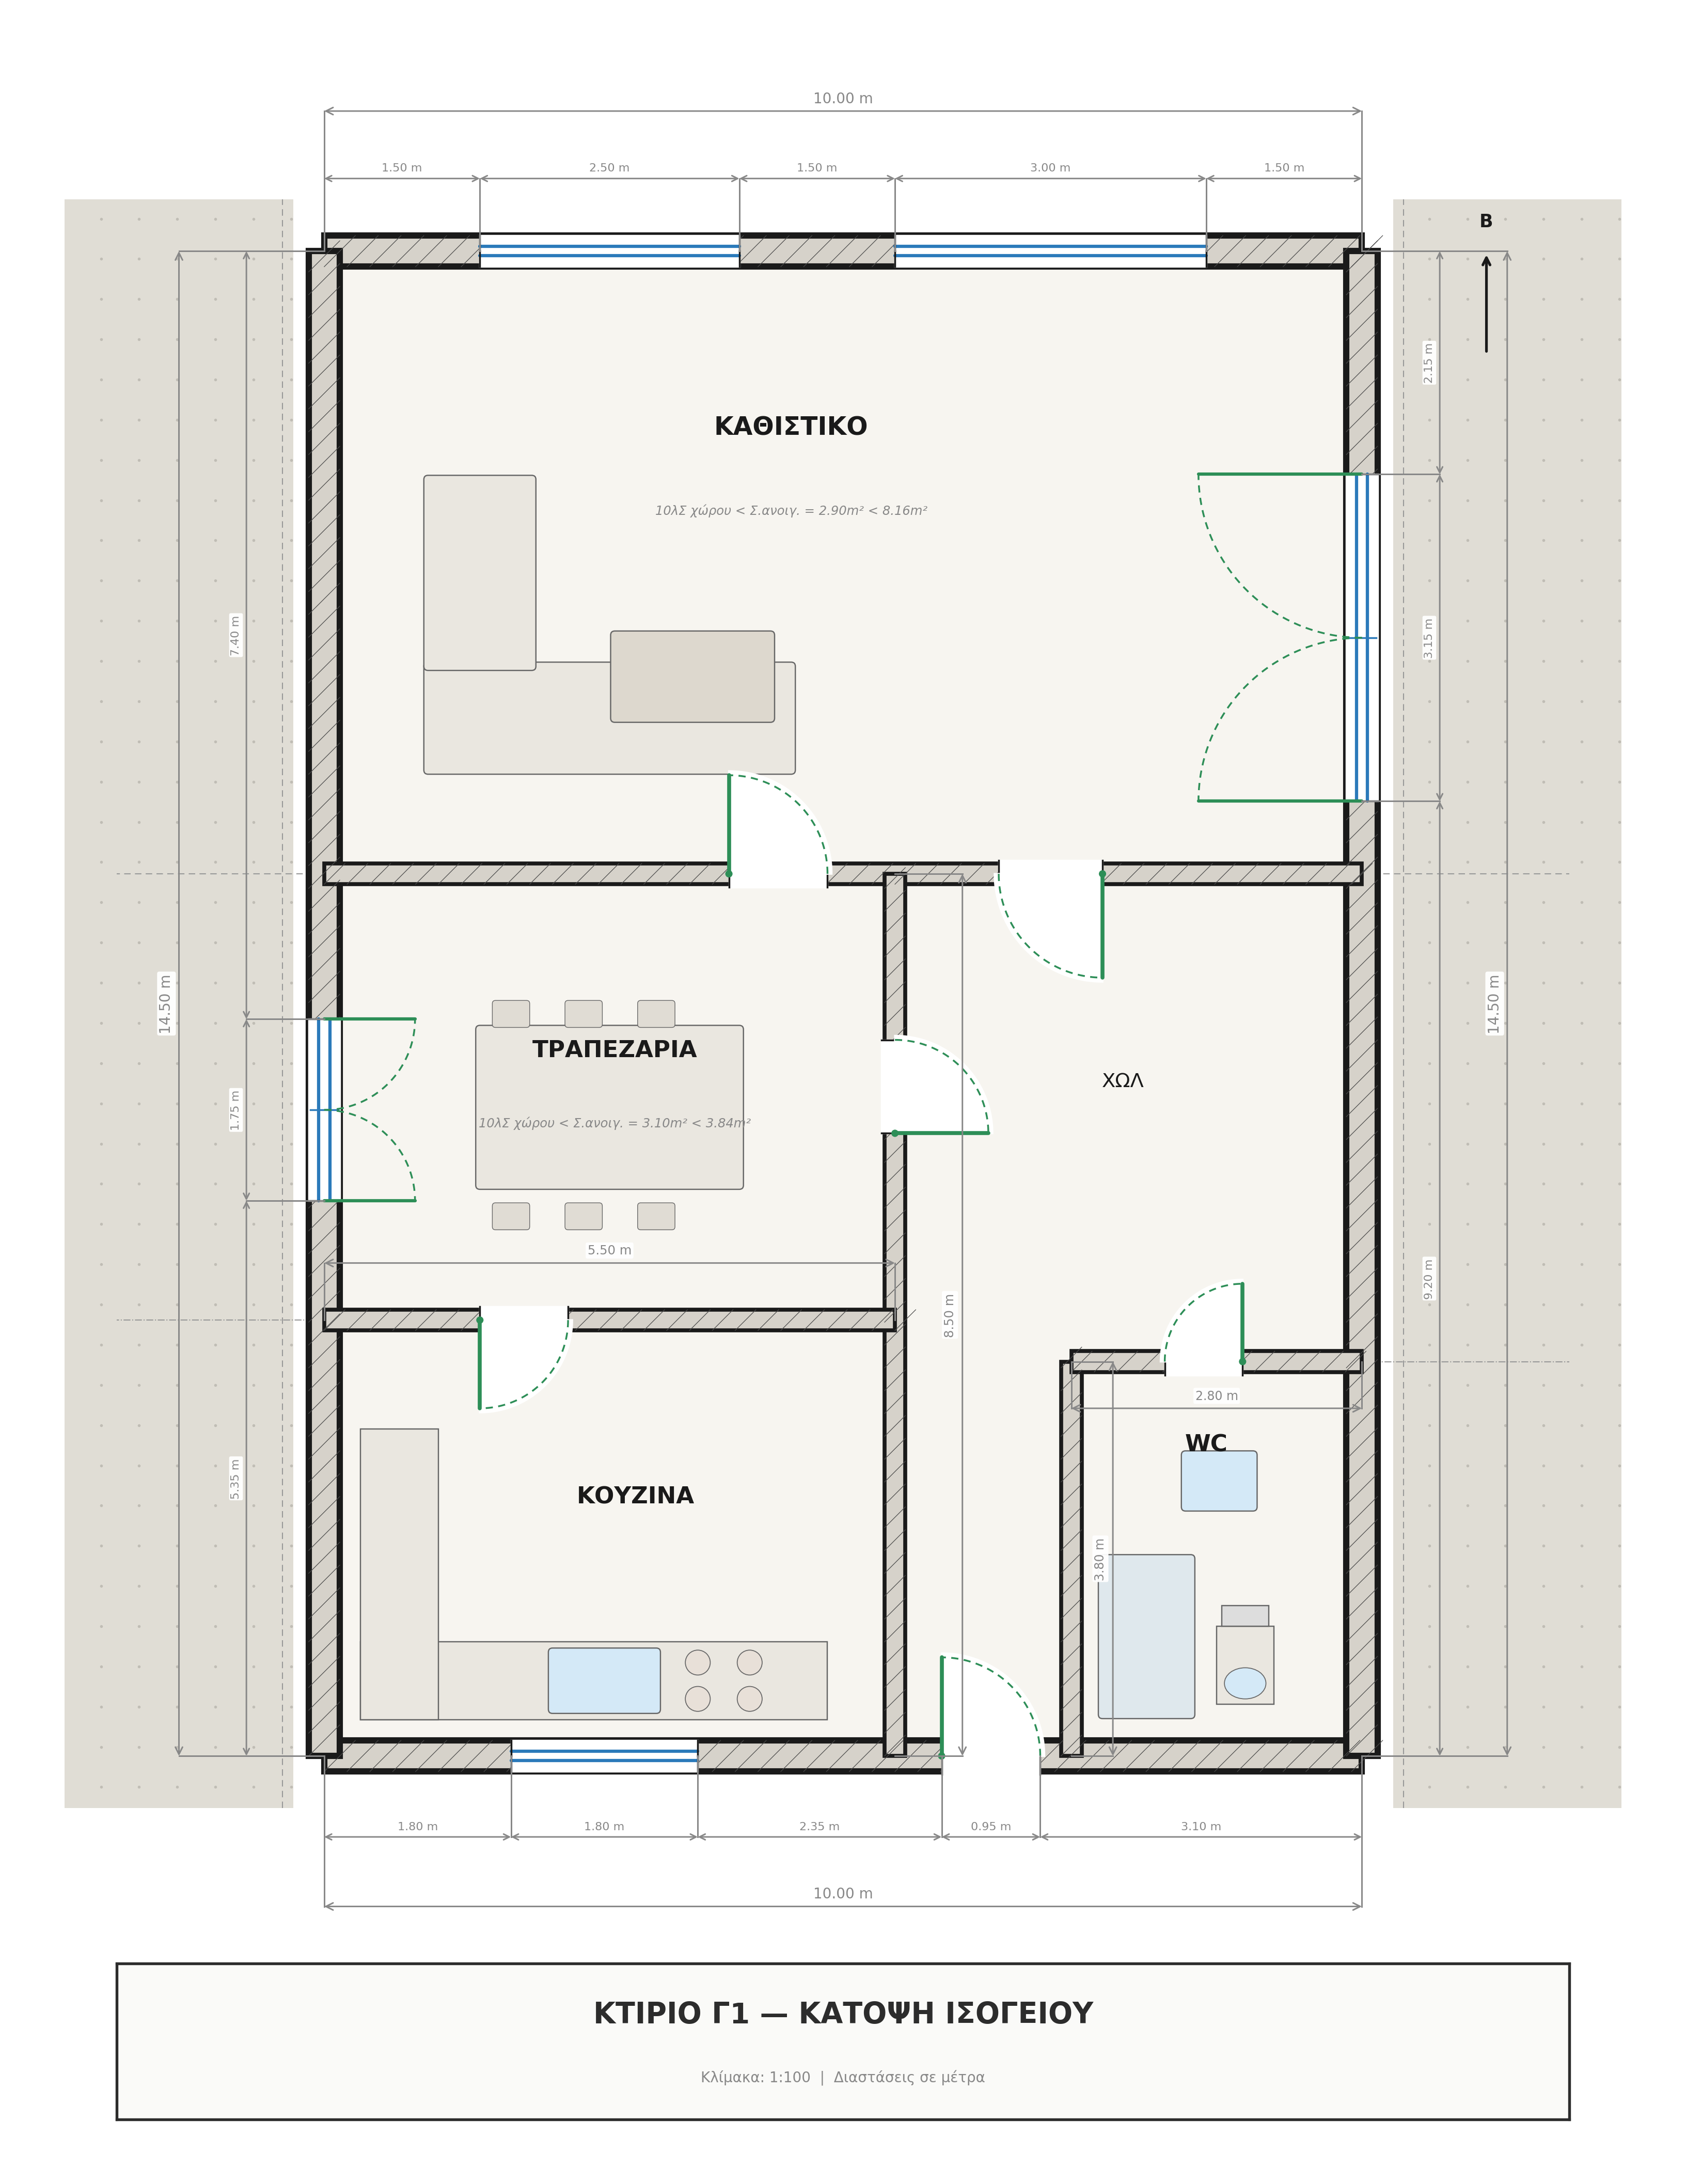
\includegraphics[width=0.84\textwidth]{floor_plan_G1.png}
\caption{Κάτοψη του Κτιρίου Γ1 που χρησιμοποιήθηκε ως βάση για την αποτύπωση του εξωτερικού περιβλήματος.}
\label{fig:floorplan}
\end{figure}

Η κάτοψη περιλαμβάνει πέντε βασικούς λειτουργικούς χώρους:

\begin{itemize}
\item καθιστικό,
\item τραπεζαρία,
\item κουζίνα,
\item WC,
\item χώλ.
\end{itemize}

\subsection{Γεωμετρικά χαρακτηριστικά της κάτοψης}

Οι βασικές γεωμετρικές πληροφορίες του κτιρίου συνοψίζονται στον επόμενο πίνακα.

\begin{table}[H]
\centering
\caption{Γενικά γεωμετρικά στοιχεία κτιρίου}
\begin{tabularx}{\textwidth}{L C{3.2cm}}
\toprule
\textbf{Μέγεθος} & \textbf{Τιμή} \\
\midrule
Συνολικές εξωτερικές διαστάσεις κάτοψης & \(10.00 \times 14.50\,\mathrm{m}\) \\
Συνολικό εμβαδόν δαπέδου / οροφής & \(145.00\,\mathrm{m^2}\) \\
Ύψος ορόφου & \(3.00\,\mathrm{m}\) \\
Πάχος εξωτερικών τοίχων & \(0.30\,\mathrm{m}\) \\
Πάχος εσωτερικών τοίχων & \(0.20\,\mathrm{m}\) \\
Περίμετρος κάτοψης & \(2 \times (10.00 + 14.50) = 49.00\,\mathrm{m}\) \\
\bottomrule
\end{tabularx}
\end{table}

\subsubsection{Επιμέρους εμβαδά λειτουργικών χώρων}

Με βάση τη γεωμετρία της κάτοψης, τα επιμέρους εμβαδά των χώρων υπολογίζονται ως εξής:

\begin{table}[H]
\centering
\small
\caption{Εμβαδά επιμέρους χώρων}
\begin{tabularx}{\textwidth}{L L C{2.8cm}}
\toprule
\textbf{Χώρος} & \textbf{Υπολογισμός} & \textbf{Εμβαδόν (\(\mathrm{m^2}\))} \\
\midrule
Καθιστικό & \(10.00 \times (14.50 - 8.50)\) & 60.00 \\
Τραπεζαρία & \(5.50 \times (8.50 - 4.20)\) & 23.65 \\
Κουζίνα & \(5.50 \times 4.20\) & 23.10 \\
WC & \((10.00 - 7.20) \times 3.80\) & 10.64 \\
Χώλ & \((10.00 - 5.50)\times(8.50 - 3.80) + (7.20 - 5.50)\times 3.80\) & 27.61 \\
\midrule
\textbf{Σύνολο} &  & \textbf{145.00} \\
\bottomrule
\end{tabularx}
\end{table}

Το άθροισμα των επιμέρους εμβαδών συμπίπτει με το συνολικό εμβαδόν της κάτοψης,
γεγονός που επιβεβαιώνει τη συνέπεια της γεωμετρικής αποτύπωσης.

\subsection{Προσανατολισμός του κτιρίου και ανοίγματα}

Για τις ανάγκες της μελέτης θεωρείται ότι:

\begin{itemize}
\item η άνω πλευρά της κάτοψης είναι η \textbf{βόρεια όψη},
\item η κάτω πλευρά είναι η \textbf{νότια όψη},
\item η δεξιά πλευρά είναι η \textbf{ανατολική όψη},
\item η αριστερή πλευρά είναι η \textbf{δυτική όψη}.
\end{itemize}

Από την κάτοψη προκύπτουν τα ακόλουθα διαφανή στοιχεία του εξωτερικού περιβλήματος:

\begin{table}[H]
\centering
\small
\caption{Ανοίγματα ανά όψη}
\begin{tabularx}{\textwidth}{L C{2.7cm} C{2.2cm} C{2.2cm} C{2.4cm}}
\toprule
\textbf{Άνοιγμα} & \textbf{Προσανατολισμός} & \textbf{Πλάτος (m)} & \textbf{Ύψος (m)} & \textbf{Εμβαδόν (\(\mathrm{m^2}\))} \\
\midrule
Παράθυρο Π1 -- Καθιστικό & Βορράς & 2.50 & 1.40 & 3.50 \\
Παράθυρο Π2 -- Καθιστικό & Βορράς & 3.00 & 1.40 & 4.20 \\
Παράθυρο Π3 -- Κουζίνα & Νότος & 1.80 & 1.40 & 2.52 \\
Μπαλκονόπορτα -- Καθιστικό & Ανατολή & 3.15 & 2.40 & 7.56 \\
Μπαλκονόπορτα -- Τραπεζαρία & Δύση & 1.75 & 2.40 & 4.20 \\
\midrule
\textbf{Σύνολο} &  &  &  & \textbf{21.98} \\
\bottomrule
\end{tabularx}
\end{table}

Οι απλές παραθυρικές επιφάνειες θεωρήθηκαν με ύψος \(1.40\,\mathrm{m}\), ενώ οι
μπαλκονόπορτες με ύψος \(2.40\,\mathrm{m}\). Η παραδοχή αυτή κρίθηκε αναγκαία, καθώς η
διαθέσιμη πληροφορία προέρχεται από κάτοψη και όχι από όψη του κτιρίου.

\subsection{Υποδήλωση ονομασίας δομικών στοιχείων}

Στο παρόν βήμα καταγράφονται αναλυτικά τα δομικά στοιχεία του εξωτερικού περιβλήματος
με τον αντίστοιχο συμβολισμό, τον προσανατολισμό τους, τη γεωμετρία τους και τις
επιφάνειές τους.

\subsubsection{Πίνακας Βήμα 1α -- Καταγραφή δομικών στοιχείων εξωτερικού περιβλήματος}

Για πληρότητα, παρατίθεται και ο συγκεντρωτικός πίνακας του Βήματος 1α, ο οποίος
αποτελεί την πλήρη απογραφή των αδιαφανών και διαφανών στοιχείων του κελύφους.

\begin{table}[H]
\centering
\scriptsize
\caption{Βήμα 1α -- Καταγραφή δομικών στοιχείων εξωτερικού περιβλήματος}
\resizebox{\textwidth}{!}{%
\begin{tabular}{p{1.9cm}p{2.8cm}p{4.2cm}p{2.3cm}p{2.2cm}p{1.5cm}p{1.8cm}p{1.7cm}p{2.0cm}}
\toprule
\textbf{Συμβολισμός} & \textbf{Τύπος στοιχείου} & \textbf{Υλικά κατασκευής} & \textbf{Προσανατολισμός} & \textbf{Μήκος/πλάτος (m)} & \textbf{Ύψος (m)} & \textbf{Επιφάνεια (\(\mathrm{m^2}\))} & \textbf{Αριθμός επιφανειών} & \textbf{Συντ. θερμοπερατότητας \(\mathrm{W/(m^2K)}\)} \\
\midrule
\multicolumn{9}{l}{\textbf{Αδιαφανή στοιχεία}} \\
\midrule
\(W_{L\mathrm{B}}\) & Εξωτερικός τοίχος & Τούβλο / μόνωση / σκυρόδεμα / επίχρισμα & Βορράς (Β) & 10.00 & 3.00 & 22.30 & 1 & 0.40 \\
\(W_{L\mathrm{N}}\) & Εξωτερικός τοίχος & Τούβλο / μόνωση / σκυρόδεμα / επίχρισμα & Νότος (Ν) & 10.00 & 3.00 & 27.48 & 1 & 0.40 \\
\(W_{L\mathrm{A}}\) & Εξωτερικός τοίχος & Τούβλο / μόνωση / σκυρόδεμα / επίχρισμα & Ανατολή (Α) & 14.50 & 3.00 & 35.94 & 1 & 0.40 \\
\(W_{L\Delta}\) & Εξωτερικός τοίχος & Τούβλο / μόνωση / σκυρόδεμα / επίχρισμα & Δύση (Δ) & 14.50 & 3.00 & 39.30 & 1 & 0.40 \\
\(R\) & Οροφή -- επαφή με εξωτερικό αέρα & Ο.Σ. / μόνωση / ασφαλτική επικάλυψη & -- & 10.00 \(\times\) 14.50 & -- & 145.00 & 1 & 0.35 \\
\(F\) & Δάπεδο -- επαφή με το έδαφος & Ο.Σ. / μόνωση / πλακάκι & -- & 10.00 \(\times\) 14.50 & -- & 145.00 & 1 & 0.60 \\
\midrule
\multicolumn{9}{l}{\textbf{Διαφανή στοιχεία}} \\
\midrule
\(W_{i\mathrm{B}1}\) & Παράθυρο -- καθιστικό & Αλουμίνιο / διπλό τζάμι & Βορράς (Β) & 2.50 & 1.40 & 3.50 & 1 & 2.40 \\
\(W_{i\mathrm{B}2}\) & Παράθυρο -- καθιστικό & Αλουμίνιο / διπλό τζάμι & Βορράς (Β) & 3.00 & 1.40 & 4.20 & 1 & 2.40 \\
\(W_{i\mathrm{N}}\) & Παράθυρο -- κουζίνα & Αλουμίνιο / διπλό τζάμι & Νότος (Ν) & 1.80 & 1.40 & 2.52 & 1 & 2.40 \\
\(W_{i\mathrm{A}}\) & Μπαλκονόπορτα (δίφυλλη) -- καθιστικό & Αλουμίνιο / διπλό τζάμι & Ανατολή (Α) & 3.15 & 2.40 & 7.56 & 1 & 2.40 \\
\(W_{i\Delta}\) & Μπαλκονόπορτα (δίφυλλη) -- τραπεζαρία & Αλουμίνιο / διπλό τζάμι & Δύση (Δ) & 1.75 & 2.40 & 4.20 & 1 & 2.40 \\
\midrule
\multicolumn{6}{r}{\textbf{Σύνολο αδιαφανών επιφανειών}} & \textbf{415.02} & \multicolumn{2}{l}{} \\
\multicolumn{6}{r}{\textbf{Σύνολο διαφανών επιφανειών}} & \textbf{21.98} & \multicolumn{2}{l}{} \\
\bottomrule
\end{tabular}%
}
\end{table}

\noindent Ο παραπάνω πίνακας είναι η πλήρης μορφή της καταγραφής του εξωτερικού
περιβλήματος. Για λόγους αναγνωσιμότητας, στη συνέχεια η ίδια πληροφορία αναλύεται
και σε επιμέρους πίνακες αδιαφανών και διαφανών στοιχείων.

\subsubsection{Αδιαφανή στοιχεία}

\begin{table}[H]
\centering
\small
\caption{Αδιαφανή δομικά στοιχεία του κτιρίου}
\begin{tabularx}{\textwidth}{C{2.6cm} L C{2.2cm} C{3.0cm} C{2.4cm}}
\toprule
\textbf{Συμβολισμός} & \textbf{Στοιχείο} & \textbf{Όψη} & \textbf{Διαστάσεις} & \textbf{Επιφάνεια (\(\mathrm{m^2}\))} \\
\midrule
\(W_{L\mathrm{B}}\) & Εξωτερικός τοίχος & Βορράς & \(10.00 \times 3.00\) & 22.30 \\
\(W_{L\mathrm{N}}\) & Εξωτερικός τοίχος & Νότος & \(10.00 \times 3.00\) & 27.48 \\
\(W_{L\mathrm{A}}\) & Εξωτερικός τοίχος & Ανατολή & \(14.50 \times 3.00\) & 35.94 \\
\(W_{L\Delta}\) & Εξωτερικός τοίχος & Δύση & \(14.50 \times 3.00\) & 39.30 \\
\(R\) & Οροφή σε επαφή με εξωτερικό αέρα & -- & \(10.00 \times 14.50\) & 145.00 \\
\(F\) & Δάπεδο σε επαφή με το έδαφος & -- & \(10.00 \times 14.50\) & 145.00 \\
\bottomrule
\end{tabularx}
\end{table}

\subsubsection{Διαφανή στοιχεία}

\begin{table}[H]
\centering
\small
\caption{Διαφανή δομικά στοιχεία του κτιρίου}
\begin{tabularx}{\textwidth}{C{2.6cm} L C{2.3cm} C{3.0cm} C{2.4cm}}
\toprule
\textbf{Συμβολισμός} & \textbf{Στοιχείο} & \textbf{Όψη} & \textbf{Διαστάσεις} & \textbf{Επιφάνεια (\(\mathrm{m^2}\))} \\
\midrule
\(W_{i\mathrm{B}1}\) & Παράθυρο καθιστικού & Βορράς & \(2.50 \times 1.40\) & 3.50 \\
\(W_{i\mathrm{B}2}\) & Παράθυρο καθιστικού & Βορράς & \(3.00 \times 1.40\) & 4.20 \\
\(W_{i\mathrm{N}}\) & Παράθυρο κουζίνας & Νότος & \(1.80 \times 1.40\) & 2.52 \\
\(W_{i\mathrm{A}}\) & Μπαλκονόπορτα καθιστικού & Ανατολή & \(3.15 \times 2.40\) & 7.56 \\
\(W_{i\Delta}\) & Μπαλκονόπορτα τραπεζαρίας & Δύση & \(1.75 \times 2.40\) & 4.20 \\
\bottomrule
\end{tabularx}
\end{table}

\subsection{Υπολογισμός επιφανειών εξωτερικού περιβλήματος}

\subsubsection{Ακαθάριστες επιφάνειες εξωτερικών τοίχων}

Οι ακαθάριστες επιφάνειες των τοίχων προκύπτουν από το μήκος κάθε όψης επί το ύψος:

\[
A_{\text{Β,ακ.}} = 10.00 \times 3.00 = 30.00\,\mathrm{m^2}
\]
\[
A_{\text{Ν,ακ.}} = 10.00 \times 3.00 = 30.00\,\mathrm{m^2}
\]
\[
A_{\text{Α,ακ.}} = 14.50 \times 3.00 = 43.50\,\mathrm{m^2}
\]
\[
A_{\Delta,\text{ακ.}} = 14.50 \times 3.00 = 43.50\,\mathrm{m^2}
\]

Άρα:

\[
A_{\text{τοίχων,ακ.}} = 30.00 + 30.00 + 43.50 + 43.50 = 147.00\,\mathrm{m^2}
\]

\subsubsection{Καθαρές επιφάνειες εξωτερικών τοίχων}

Οι καθαρές επιφάνειες προκύπτουν αφαιρώντας τα ανοίγματα από κάθε όψη:

\[
A_{\text{καθ.}} = A_{\text{ακ.}} - \sum A_{\text{ανοιγμ.}}
\]

Αναλυτικά:

\[
A_{\text{Β,καθ.}} = 30.00 - (3.50 + 4.20) = 22.30\,\mathrm{m^2}
\]
\[
A_{\text{Ν,καθ.}} = 30.00 - 2.52 = 27.48\,\mathrm{m^2}
\]
\[
A_{\text{Α,καθ.}} = 43.50 - 7.56 = 35.94\,\mathrm{m^2}
\]
\[
A_{\Delta,\text{καθ.}} = 43.50 - 4.20 = 39.30\,\mathrm{m^2}
\]

\begin{table}[H]
\centering
\small
\caption{Συγκεντρωτικός πίνακας ακαθάριστων και καθαρών επιφανειών}
\begin{tabularx}{\textwidth}{L C{2.4cm} C{2.4cm} C{2.4cm} C{2.4cm}}
\toprule
\textbf{Όψη} & \textbf{Ακαθ. επιφάνεια} & \textbf{Ανοίγματα} & \textbf{Καθαρή επιφάνεια} & \textbf{Ποσοστό ανοιγμάτων} \\
\midrule
Βορράς & 30.00 & 7.70 & 22.30 & 25.67\% \\
Νότος & 30.00 & 2.52 & 27.48 & 8.40\% \\
Ανατολή & 43.50 & 7.56 & 35.94 & 17.38\% \\
Δύση & 43.50 & 4.20 & 39.30 & 9.66\% \\
\midrule
\textbf{Σύνολο} & \textbf{147.00} & \textbf{21.98} & \textbf{125.02} & \textbf{14.95\%} \\
\bottomrule
\end{tabularx}
\end{table}

\subsection{Συντελεστές θερμοπερατότητας δομικών στοιχείων}

Με βάση τον πίνακα συντελεστών θερμοπερατότητας του Κ.Εν.Α.Κ. για τη Ζώνη Γ',
υιοθετούνται οι παρακάτω τιμές:

\begin{table}[H]
\centering
\caption{Συντελεστές θερμοπερατότητας δομικών στοιχείων}
\begin{tabularx}{\textwidth}{L C{3.4cm}}
\toprule
\textbf{Δομικό στοιχείο} & \textbf{\(U\) [\(\mathrm{W/(m^2K)}\)]} \\
\midrule
Εξωτερικός τοίχος σε επαφή με εξωτερικό αέρα & 0.40 \\
Οροφή σε επαφή με εξωτερικό αέρα & 0.35 \\
Κούφωμα / άνοιγμα σε επαφή με εξωτερικό αέρα & 2.40 \\
\bottomrule
\end{tabularx}
\end{table}

Από τον πίνακα αυτό γίνεται άμεσα αντιληπτό ότι τα κουφώματα αποτελούν το θερμικά
ασθενέστερο τμήμα του κελύφους, καθώς ο συντελεστής τους είναι πολλαπλάσιος εκείνου
των αδιαφανών στοιχείων.

Για την εφαρμογή της μεθόδου \textenglish{ASHRAE CLTD/CLF} στο επόμενο στάδιο της
εργασίας, οι εξωτερικοί τοίχοι προσεγγίζονται ως τοίχοι της \textbf{Ομάδας D}
(\textenglish{Group D}), δηλαδή ως δομικά στοιχεία \textbf{μεσαίου θερμικού βάρους}.
Η επιλογή αυτή είναι συμβατή με την παραδοχή κατασκευής τύπου τοιχοποιίας / σκυροδέματος
με θερμομόνωση και με τη συνολική θερμική συμπεριφορά που αποδόθηκε στο κέλυφος.

\subsection{Υπολογισμός μέσου συντελεστή θερμοπερατότητας Um}

Για το εξωτερικό κέλυφος που θα χρησιμοποιηθεί άμεσα στους θερινούς υπολογισμούς
(καθαροί εξωτερικοί τοίχοι, οροφή και διαφανή στοιχεία), ο μέσος συντελεστής
θερμοπερατότητας λαμβάνεται ως ο σταθμισμένος μέσος των αντίστοιχων επιφανειών:

\[
U_m = \frac{\sum U_i A_i}{\sum A_i}
\]

Στην παρούσα περίπτωση:

\[
U_m =
\frac{
0.40 \times 125.02 +
0.35 \times 145.00 +
2.40 \times 21.98
}{
125.02 + 145.00 + 21.98
}
\]

\[
U_m =
\frac{50.008 + 50.750 + 52.752}{292.00}
=
\frac{153.510}{292.00}
=
0.526\,\mathrm{W/(m^2K)}
\]

Άρα, με στρογγυλοποίηση δύο δεκαδικών ψηφίων:

\[
\boxed{U_m \approx 0.53\,\mathrm{W/(m^2K)}}
\]

Η τιμή αυτή εκφράζει τη μέση θερμοπερατότητα του εξωτερικού κελύφους που λαμβάνεται
υπόψη στους μετέπειτα υπολογισμούς ψυκτικού φορτίου και δίνει μία συνολική εικόνα του
θερμικού επιπέδου προστασίας του κτιρίου.

\subsection{Συνοπτική αποτίμηση του κτιρίου προς μελέτη}

Από την ανάλυση του Κτιρίου Γ1 προκύπτουν τα ακόλουθα βασικά συμπεράσματα:

\begin{itemize}
\item το κτίριο έχει συνολικό εμβαδόν \(145.00\,\mathrm{m^2}\) και ύψος \(3.00\,\mathrm{m}\),
\item το συνολικό ακαθάριστο εμβαδόν εξωτερικών τοίχων είναι \(147.00\,\mathrm{m^2}\),
\item το συνολικό καθαρό εμβαδόν εξωτερικών τοίχων είναι \(125.02\,\mathrm{m^2}\),
\item το συνολικό εμβαδόν ανοιγμάτων είναι \(21.98\,\mathrm{m^2}\),
\item η οροφή έχει επιφάνεια \(145.00\,\mathrm{m^2}\),
\item οι συντελεστές θερμοπερατότητας που θα χρησιμοποιηθούν στη συνέχεια είναι
\(U_{\text{τοίχου}} = 0.40\), \(U_{\text{οροφής}} = 0.35\) και
\(U_{\text{ανοιγμάτων}} = 2.40\,\mathrm{W/(m^2K)}\),
\item ο μέσος συντελεστής θερμοπερατότητας του προς μελέτη κελύφους είναι
\(U_m \approx 0.53\,\mathrm{W/(m^2K)}\).
\end{itemize}

Με τα δεδομένα αυτά ολοκληρώνεται η τεκμηρίωση των Sections 1, 2 και 3 του
τελικού report και διαμορφώνεται το απαραίτητο υπόβαθρο για το Section 4. Στην
επόμενη ενότητα ακολουθεί ο πλήρης υπολογισμός των ψυκτικών φορτίων με τη μέθοδο
CLTD της ASHRAE για τις ζητούμενες ώρες της 21ης Ιουλίου.

\clearpage
\section{Υπολογισμός ψυκτικών φορτίων}

\subsection{Μεθοδολογία υπολογισμού}

Για τον υπολογισμό των ψυκτικών φορτίων χρησιμοποιείται η μέθοδος
\textenglish{ASHRAE CLTD/CLF}. Η μέθοδος αυτή αποτελεί κλασική προσεγγιστική τεχνική
υπολογισμού θερινών φορτίων, η οποία ενσωματώνει:

\begin{itemize}
\item τη θερμική αδράνεια των αδιαφανών δομικών στοιχείων μέσω των τιμών
\textenglish{CLTD} (\textenglish{Cooling Load Temperature Difference}),
\item τη χρονική υστέρηση των ηλιακών και εσωτερικών κερδών μέσω των
\textenglish{CLF} (\textenglish{Cooling Load Factor}),
\item και τον προσανατολισμό των ανοιγμάτων μέσω των
\textenglish{SHGF} (\textenglish{Solar Heat Gain Factor}).
\end{itemize}

Ο υπολογισμός πραγματοποιείται για την \textbf{21η Ιουλίου} και για τις ώρες
\textbf{08:00, 12:00, 16:00, 20:00 και 24:00}, όπως ζητείται στην εκφώνηση. Η
κατοικία εξετάζεται ως \textbf{μία ενιαία θερμική ζώνη}.

\subsubsection{Βασικές εξισώσεις}

\paragraph{Αδιαφανή στοιχεία (τοίχοι και οροφή)}
Για τους εξωτερικούς τοίχους χρησιμοποιείται:

\[
q_{\text{τοίχου}} = U \cdot A \cdot (CLTD)_{\text{corr}}
\]

με:

\[
(CLTD)_{\text{corr, τοίχου}} =
(CLTD + LM)\cdot K + (25.5 - T_i) + (T_{o,\mathrm{mean}} - 29.4)
\]

Για την οροφή χρησιμοποιείται:

\[
q_{\text{οροφής}} = U \cdot A \cdot (CLTD)_{\text{corr}} \cdot f
\]

με:

\[
(CLTD)_{\text{corr, οροφής}} =
(CLTD + LM)\cdot K + (25.5 - T_i) + (T_{o,\mathrm{mean}} - 29.4)
\]

\paragraph{Υαλοπίνακες λόγω αγωγής}
Για την αγωγιμότητα των υαλοπινάκων χρησιμοποιείται:

\[
q_{\text{υαλ., αγωγ.}} = U \cdot A \cdot (CLTD)_{\text{corr}}
\]

όπου:

\[
(CLTD)_{\text{corr, υαλ.}} = CLTD + (25.5 - T_i) + (T_{o,\mathrm{mean}} - 29.4)
\]

\paragraph{Ηλιακά κέρδη από παράθυρα}

\[
q_{\text{ηλιακό}} = A \cdot SC \cdot (SHGF)_{\max} \cdot CLF
\]

\paragraph{Εσωτερικά φορτία}
Για τα αισθητά φορτία ανθρώπων:

\[
q_{\text{ανθρ., αισθ.}} = N \cdot HG_{\text{sens}} \cdot CLF
\]

Για τα λανθάνοντα φορτία ανθρώπων:

\[
q_{\text{ανθρ., λανθ.}} = N \cdot HG_{\text{lat}}
\]

Για τον φωτισμό:

\[
HG_{\text{φωτ.}} = P \cdot f_u \cdot f_s
\qquad \text{και} \qquad
q_{\text{φωτ.}} = HG_{\text{φωτ.}} \cdot CLF
\]

Για τον εξοπλισμό:

\[
q_{\text{εξοπλ., αισθ.}} = HG_{\text{sens}} \cdot CLF
\qquad \text{και} \qquad
q_{\text{εξοπλ., λανθ.}} = HG_{\text{lat}}
\]

\paragraph{Αερισμός / διείσδυση}
Το αισθητό φορτίο αερισμού υπολογίζεται από:

\[
q_{\text{αερ., αισθ.}} = \dot{m}\, C_p\, (T_o - T_i)
\]

ενώ το λανθάνον φορτίο αερισμού από:

\[
q_{\text{αερ., λανθ.}} = \dot{m}\, (W_o - W_i)\, h_g
\]

\subsection{Δεδομένα σχεδιασμού και παραδοχές}

\subsubsection{Συνθήκες σχεδιασμού}

\begin{table}[H]
\centering
\caption{Κλιματικά και εσωτερικά δεδομένα σχεδιασμού}
\begin{tabularx}{\textwidth}{L C{3.8cm}}
\toprule
\textbf{Μέγεθος} & \textbf{Τιμή} \\
\midrule
Ημερομηνία υπολογισμού & 21 Ιουλίου \\
Τοποθεσία & Θεσσαλονίκη \\
Γεωγραφικό πλάτος & \(40^\circ \mathrm{N}\) \\
Εσωτερική θερμοκρασία σχεδιασμού \(T_i\) & \(26.0\,^\circ\mathrm{C}\) \\
Εσωτερική σχετική υγρασία & 50\% \\
Μέγιστη εξωτερική θερμοκρασία \(T_{o,\max}\) & \(36.0\,^\circ\mathrm{C}\) \\
Ημερήσια διακύμανση \(DR\) & \(11.0\,^\circ\mathrm{C}\) \\
Μέση εξωτερική θερμοκρασία \(T_{o,\mathrm{mean}}\) & \(30.5\,^\circ\mathrm{C}\) \\
Λόγος υγρασίας εσωτερικού αέρα \(W_i\) & \(0.0105\,\mathrm{kg_w/kg_{da}}\) \\
Λόγος υγρασίας εξωτερικού αέρα \(W_o\) & \(0.0145\,\mathrm{kg_w/kg_{da}}\) \\
\bottomrule
\end{tabularx}
\end{table}

\subsubsection{Επιλογές πινάκων και παραμέτρων της ASHRAE}

\begin{table}[H]
\centering
\caption{Επιλογές μοντέλου CLTD/CLF}
\begin{tabularx}{\textwidth}{L C{4.0cm}}
\toprule
\textbf{Παράμετρος} & \textbf{Επιλογή} \\
\midrule
Τοίχοι CLTD & Ομάδα D (\textenglish{Group D}) \\
Οροφή CLTD & Τύπος 9 χωρίς ψευδοροφή \\
Χρώμα τοίχων & Ανοιχτόχρωμοι, \(K=0.65\) \\
Χρώμα οροφής & Μέση/σκούρα, \(K=1.0\) \\
Συντελεστής ροής αέρα στην οροφή & \(f = 1.0\) \\
Διόρθωση γεωγρ. πλάτους τοίχων & \(LM \approx 0.0\) \\
Διόρθωση γεωγρ. πλάτους οροφής & \(LM_{\mathrm{HOR}} = 0.5\) \\
Συντελεστής σκίασης υαλοπινάκων & \(SC = 0.69\) \\
Εσωτερικά φορτία ανθρώπων / φωτισμού / εξοπλισμού & \(CLF = 1.0\) \\
\bottomrule
\end{tabularx}
\end{table}

\subsubsection{Κοινή διόρθωση θερμοκρασίας}

Η κοινή διόρθωση θερμοκρασίας που εισέρχεται στις εξισώσεις τοίχων, οροφής και
υαλοπινάκων είναι:

\[
(25.5 - T_i) + (T_{o,\mathrm{mean}} - 29.4)
=
(25.5 - 26.0) + (30.5 - 29.4)
=
0.6\,^\circ\mathrm{C}
\]

Άρα:

\begin{itemize}
\item για τους τοίχους:
\[
(CLTD)_{\text{corr}} = (CLTD + LM)\cdot 0.65 + 0.6
\]
\item για την οροφή:
\[
(CLTD)_{\text{corr}} = (CLTD + 0.5)\cdot 1.0 + 0.6
\]
\item για τα ανοίγματα λόγω αγωγής:
\[
(CLTD)_{\text{corr}} = CLTD + 0.6
\]
\end{itemize}

\subsubsection{Εσωτερικά φορτία και αερισμός}

\begin{table}[H]
\centering
\caption{Παραδοχές εσωτερικών φορτίων και αερισμού}
\begin{tabularx}{\textwidth}{L C{4.3cm}}
\toprule
\textbf{Παράμετρος} & \textbf{Τιμή} \\
\midrule
Αριθμός ατόμων & 4 \\
Αισθητό φορτίο ανά άτομο & \(73\,\mathrm{W/άτομο}\) \\
Λανθάνον φορτίο ανά άτομο & \(59\,\mathrm{W/άτομο}\) \\
Εγκατεστημένη ισχύς φωτισμού & \(1450\,\mathrm{W}\) \\
Συντελεστής χρήσης φωτισμού \(f_u\) & 0.30 \\
Συντελεστής φωτιστικών \(f_s\) & 1.0 \\
Αισθητό φορτίο εξοπλισμού & \(400\,\mathrm{W}\) \\
Λανθάνον φορτίο εξοπλισμού & \(200\,\mathrm{W}\) \\
Εναλλαγές αέρα ανά ώρα & \(0.5\,\mathrm{ACH}\) \\
Όγκος κτιρίου & \(145 \times 3 = 435\,\mathrm{m^3}\) \\
Παροχή αέρα & \(0.0604\,\mathrm{m^3/s} = 60.4\,\mathrm{L/s}\) \\
Μαζική παροχή αέρα & \(\dot m = 0.0727\,\mathrm{kg/s}\) \\
\bottomrule
\end{tabularx}
\end{table}

\subsubsection{Ωριαίες εξωτερικές συνθήκες}

\begin{table}[H]
\centering
\caption{Ωριαίες εξωτερικές συνθήκες για τις ώρες υπολογισμού}
\begin{tabular}{lccccc}
\toprule
\textbf{Μέγεθος} & \textbf{08:00} & \textbf{12:00} & \textbf{16:00} & \textbf{20:00} & \textbf{24:00} \\
\midrule
\(T_o\) \([\!^\circ\mathrm{C}]\) & 26.8 & 33.5 & 35.7 & 30.8 & 27.0 \\
\(\Delta T = T_o - T_i\) \([\!^\circ\mathrm{C}]\) & 0.8 & 7.5 & 9.7 & 4.8 & 1.0 \\
\bottomrule
\end{tabular}
\end{table}

\subsection{Αισθητά ψυκτικά φορτία}

\subsubsection{Φορτία από εξωτερικούς τοίχους}

Τα φορτία μέσω των τοίχων υπολογίστηκαν ξεχωριστά για κάθε προσανατολισμό, ώστε να
ληφθεί υπόψη η διαφορετική ηλιακή επιβάρυνση της κάθε όψης. Τα αποτελέσματα
φαίνονται στον ακόλουθο πίνακα.

\begin{table}[H]
\centering
\caption{Αισθητά φορτία από εξωτερικούς τοίχους}
\resizebox{\textwidth}{!}{%
\begin{tabular}{lccccc}
\toprule
\textbf{Στοιχείο} & \textbf{08:00} & \textbf{12:00} & \textbf{16:00} & \textbf{20:00} & \textbf{24:00} \\
\midrule
Τοίχος Βορράς & 21.6 & 34.3 & 37.8 & 37.8 & 30.9 \\
Τοίχος Νότος & 30.2 & 73.8 & 65.9 & 50.2 & 42.3 \\
Τοίχος Ανατολή & 128.2 & 118.0 & 81.5 & 65.6 & 61.0 \\
Τοίχος Δύση & 43.2 & 43.2 & 134.1 & 145.3 & 111.6 \\
\midrule
\textbf{Σύνολο τοίχων [W]} & \textbf{223.1} & \textbf{269.2} & \textbf{319.3} & \textbf{299.0} & \textbf{245.7} \\
\bottomrule
\end{tabular}%
}
\end{table}

Παρατηρείται ότι:

\begin{itemize}
\item η \textbf{ανατολική όψη} εμφανίζει το υψηλότερο φορτίο το πρωί, με
\(128.2\,\mathrm{W}\) στις 08:00,
\item η \textbf{δυτική όψη} εμφανίζει το υψηλότερο φορτίο το απόγευμα και το βράδυ,
με μέγιστη τιμή \(145.3\,\mathrm{W}\) στις 20:00,
\item η συνολική συνεισφορά των τοίχων παραμένει σχετικά μικρή, γεγονός που
οφείλεται στη χαμηλή τιμή \(U = 0.40\,\mathrm{W/(m^2K)}\).
\end{itemize}

\subsubsection{Φορτία από οροφή}

Η οροφή, λόγω της μεγάλης επιφάνειάς της και της άμεσης έκθεσης στην ηλιακή
ακτινοβολία, αποτελεί ιδιαίτερα σημαντική συνιστώσα του αισθητού φορτίου.

\begin{table}[H]
\centering
\caption{Αισθητό φορτίο από οροφή}
\begin{tabular}{lccccc}
\toprule
\textbf{Στοιχείο} & \textbf{08:00} & \textbf{12:00} & \textbf{16:00} & \textbf{20:00} & \textbf{24:00} \\
\midrule
Οροφή Τύπου 9 [W] & 167.5 & 477.1 & 847.5 & 817.1 & 507.5 \\
\bottomrule
\end{tabular}
\end{table}

Η μέγιστη τιμή εμφανίζεται στις \textbf{16:00} και όχι στο μεσημέρι. Αυτό είναι
χαρακτηριστική συνέπεια της \textbf{θερμικής αδράνειας} της βαριάς οροφής: η
θερμότητα που απορροφάται κατά τις προηγούμενες ώρες αποδίδεται με χρονική υστέρηση
στο εσωτερικό.

\subsubsection{Φορτία από υαλοπίνακες λόγω αγωγής}

Τα φορτία από αγωγιμότητα των υαλοπινάκων υπολογίστηκαν με την ειδική τιμή
\((CLTD)_{\text{corr}} = CLTD + 0.6\).

\begin{table}[H]
\centering
\caption{Αισθητά φορτία από υαλοπίνακες λόγω αγωγής}
\resizebox{\textwidth}{!}{%
\begin{tabular}{lccccc}
\toprule
\textbf{Στοιχείο} & \textbf{08:00} & \textbf{12:00} & \textbf{16:00} & \textbf{20:00} & \textbf{24:00} \\
\midrule
Π1+Π2 Βορράς & 11.1 & 103.5 & 158.9 & 85.0 & 29.6 \\
Π3 Νότος & 3.6 & 33.9 & 52.0 & 27.8 & 9.7 \\
Μπαλκονόπορτα Ανατολής & 10.9 & 101.6 & 156.0 & 83.5 & 29.0 \\
Μπαλκονόπορτα Δύσης & 6.0 & 56.4 & 86.7 & 46.4 & 16.1 \\
\midrule
\textbf{Σύνολο αγωγής [W]} & \textbf{31.7} & \textbf{295.4} & \textbf{453.7} & \textbf{242.7} & \textbf{84.4} \\
\bottomrule
\end{tabular}%
}
\end{table}

Η αγωγή των ανοιγμάτων ακολουθεί περισσότερο τη θερμοκρασία εξωτερικού αέρα παρά την
άμεση ηλιακή ακτινοβολία, με αποτέλεσμα να κορυφώνεται στις \textbf{16:00}, όταν η
εξωτερική θερμοκρασία είναι μέγιστη.

\subsubsection{Ηλιακά κέρδη από παράθυρα και μπαλκονόπορτες}

Για τα ηλιακά κέρδη χρησιμοποιήθηκαν:

\begin{itemize}
\item \(SC = 0.69\),
\item \(SHGF_{\max}\) για \(40^\circ\mathrm{N}\) και Ιούλιο:
\[
SHGF_{\max,\mathrm{N}} = 131,\quad
SHGF_{\max,\mathrm{S}} = 190,\quad
SHGF_{\max,\mathrm{E}} = SHGF_{\max,\mathrm{W}} = 527\;\mathrm{W/m^2}
\]
\item ωριαίοι συντελεστές \(CLF\) ανά προσανατολισμό.
\end{itemize}

\begin{table}[H]
\centering
\caption{Ηλιακά κέρδη από διαφανή στοιχεία}
\resizebox{\textwidth}{!}{%
\begin{tabular}{lccccc}
\toprule
\textbf{Στοιχείο} & \textbf{08:00} & \textbf{12:00} & \textbf{16:00} & \textbf{20:00} & \textbf{24:00} \\
\midrule
Π1+Π2 Βορράς & 452.4 & 619.4 & 522.0 & 125.3 & 69.6 \\
Π3 Νότος & 76.0 & 274.2 & 115.6 & 29.7 & 16.5 \\
Μπαλκονόπορτα Ανατολής & 2199.2 & 742.2 & 467.3 & 137.5 & 82.5 \\
Μπαλκονόπορτα Δύσης & 168.0 & 259.6 & 1252.3 & 183.3 & 91.6 \\
\midrule
\textbf{Σύνολο ηλιακών κερδών [W]} & \textbf{2895.6} & \textbf{1895.5} & \textbf{2357.3} & \textbf{475.7} & \textbf{260.2} \\
\bottomrule
\end{tabular}%
}
\end{table}

Ο πίνακας αυτός δείχνει με σαφήνεια τον κυρίαρχο ρόλο των ανοιγμάτων στη θερινή
συμπεριφορά της κατοικίας:

\begin{itemize}
\item στις \textbf{08:00} κυριαρχεί η ανατολική μπαλκονόπορτα με
\(2199.2\,\mathrm{W}\), δηλαδή σχεδόν το \textbf{76\%} των συνολικών ηλιακών κερδών εκείνης της ώρας,
\item στις \textbf{16:00} κυριαρχεί η δυτική μπαλκονόπορτα με
\(1252.3\,\mathrm{W}\), δηλαδή περισσότερο από το \textbf{53\%} των ηλιακών κερδών της ώρας αιχμής,
\item τα συνολικά ηλιακά κέρδη αποτελούν τη \textbf{σημαντικότερη αισθητή συνιστώσα}
για μεγάλο μέρος της ημέρας.
\end{itemize}

\subsubsection{Εσωτερικά αισθητά φορτία}

Τα εσωτερικά αισθητά φορτία θεωρήθηκαν σταθερά στη διάρκεια της ημέρας, με
\(CLF=1.0\), ως συντηρητική παραδοχή για κατοικία.

\begin{table}[H]
\centering
\caption{Εσωτερικά αισθητά φορτία}
\begin{tabular}{lcc}
\toprule
\textbf{Πηγή φορτίου} & \textbf{Υπολογισμός} & \textbf{Φορτίο [W]} \\
\midrule
Άνθρωποι & \(4 \times 73 \times 1.0\) & 292 \\
Φωτισμός & \(1450 \times 0.30 \times 1.0 \times 1.0\) & 435 \\
Εξοπλισμός & \(400 \times 1.0\) & 400 \\
\midrule
\textbf{Σύνολο} &  & \textbf{1127} \\
\bottomrule
\end{tabular}
\end{table}

Επειδή τα φορτία αυτά παραμένουν σταθερά, η σχετική συμμετοχή τους αυξάνει σημαντικά
στις βραδινές ώρες, όταν μειώνονται τα ηλιακά και αγώγιμα φορτία.

\subsubsection{Αισθητό φορτίο αερισμού / διείσδυσης}

Από την παραδοχή \(ACH = 0.5\) προκύπτει:

\[
\dot V = \frac{145 \times 3 \times 0.5}{3600} = 0.0604\,\mathrm{m^3/s}
\]

\[
\dot m = 1.204 \times 0.0604 = 0.0727\,\mathrm{kg/s}
\]

Με \(C_p \approx 1028.15\,\mathrm{J/(kgK)}\), το αισθητό φορτίο αερισμού γίνεται:

\begin{table}[H]
\centering
\caption{Αισθητό φορτίο αερισμού}
\begin{tabular}{lccccc}
\toprule
\textbf{Μέγεθος} & \textbf{08:00} & \textbf{12:00} & \textbf{16:00} & \textbf{20:00} & \textbf{24:00} \\
\midrule
\(\Delta T = T_o - T_i\) \([\!^\circ\mathrm{C}]\) & 0.8 & 7.5 & 9.7 & 4.8 & 1.0 \\
\(q_{\text{αερ., αισθ.}}\) [W] & 56.8 & 558.7 & 723.2 & 361.2 & 73.3 \\
\bottomrule
\end{tabular}
\end{table}

Η συνεισφορά του αερισμού εξαρτάται άμεσα από τη διαφορά θερμοκρασίας
\((T_o - T_i)\), γι' αυτό και κορυφώνεται στις \textbf{16:00}.

\subsubsection{Συνολικό αισθητό φορτίο}

\begin{table}[H]
\centering
\caption{Συγκεντρωτικός πίνακας αισθητών φορτίων}
\resizebox{\textwidth}{!}{%
\begin{tabular}{lccccc}
\toprule
\textbf{Κατηγορία φορτίου} & \textbf{08:00} & \textbf{12:00} & \textbf{16:00} & \textbf{20:00} & \textbf{24:00} \\
\midrule
Τοίχοι & 223.1 & 269.2 & 319.3 & 299.0 & 245.7 \\
Οροφή & 167.5 & 477.1 & 847.5 & 817.1 & 507.5 \\
Υαλοπίνακες λόγω αγωγής & 31.7 & 295.4 & 453.7 & 242.7 & 84.4 \\
Ηλιακά κέρδη ανοιγμάτων & 2895.6 & 1895.5 & 2357.3 & 475.7 & 260.2 \\
Εσωτερικά αισθητά & 1127.0 & 1127.0 & 1127.0 & 1127.0 & 1127.0 \\
Αερισμός / διείσδυση & 56.8 & 558.7 & 723.2 & 361.2 & 73.3 \\
\midrule
\textbf{Συνολικό αισθητό φορτίο [W]} & \textbf{4501.7} & \textbf{4622.9} & \textbf{5828.0} & \textbf{3322.7} & \textbf{2298.2} \\
\bottomrule
\end{tabular}%
}
\end{table}

\subsection{Λανθάνοντα ψυκτικά φορτία}

\subsubsection{Λανθάνον φορτίο από ανθρώπους και εξοπλισμό}

\begin{table}[H]
\centering
\caption{Σταθερά λανθάνοντα φορτία}
\begin{tabular}{lcc}
\toprule
\textbf{Πηγή φορτίου} & \textbf{Υπολογισμός} & \textbf{Φορτίο [W]} \\
\midrule
Άνθρωποι & \(4 \times 59\) & 236 \\
Εξοπλισμός & Δοθείσα παραδοχή & 200 \\
\midrule
\textbf{Σύνολο} &  & \textbf{436} \\
\bottomrule
\end{tabular}
\end{table}

\subsubsection{Λανθάνον φορτίο αερισμού}

Με:

\[
\Delta W = W_o - W_i = 0.0145 - 0.0105 = 0.0040
\]

και με \(\dot m = 0.0727\,\mathrm{kg/s}\), το λανθάνον φορτίο από αερισμό είναι:

\begin{table}[H]
\centering
\caption{Λανθάνον φορτίο αερισμού}
\begin{tabular}{lccccc}
\toprule
\textbf{Μέγεθος} & \textbf{08:00} & \textbf{12:00} & \textbf{16:00} & \textbf{20:00} & \textbf{24:00} \\
\midrule
\(q_{\text{αερ., λανθ.}}\) [W] & 742.1 & 743.9 & 744.5 & 743.2 & 742.2 \\
\bottomrule
\end{tabular}
\end{table}

Η μικρή μεταβολή των τιμών οφείλεται στην πολύ περιορισμένη μεταβολή της ενθαλπίας
αναφοράς \(h_g\) από ώρα σε ώρα. Στην πράξη, το λανθάνον φορτίο αερισμού μπορεί να
θεωρηθεί σχεδόν \textbf{σταθερό} κατά τη διάρκεια της ημέρας.

\subsubsection{Συνολικό λανθάνον φορτίο}

\begin{table}[H]
\centering
\caption{Συγκεντρωτικός πίνακας λανθανόντων φορτίων}
\begin{tabular}{lccccc}
\toprule
\textbf{Κατηγορία φορτίου} & \textbf{08:00} & \textbf{12:00} & \textbf{16:00} & \textbf{20:00} & \textbf{24:00} \\
\midrule
Αερισμός / διείσδυση & 742.1 & 743.9 & 744.5 & 743.2 & 742.2 \\
Άνθρωποι & 236.0 & 236.0 & 236.0 & 236.0 & 236.0 \\
Εξοπλισμός & 200.0 & 200.0 & 200.0 & 200.0 & 200.0 \\
\midrule
\textbf{Συνολικό λανθάνον φορτίο [W]} & \textbf{1178.1} & \textbf{1179.9} & \textbf{1180.5} & \textbf{1179.2} & \textbf{1178.2} \\
\bottomrule
\end{tabular}
\end{table}

\subsection{Συγκεντρωτικά αποτελέσματα}

\begin{table}[H]
\centering
\caption{Συνολικά ψυκτικά φορτία ανά ώρα}
\begin{tabular}{lccccc}
\toprule
\textbf{Μέγεθος} & \textbf{08:00} & \textbf{12:00} & \textbf{16:00} & \textbf{20:00} & \textbf{24:00} \\
\midrule
Συνολικό αισθητό φορτίο [W] & 4501.7 & 4622.9 & 5828.0 & 3322.7 & 2298.2 \\
Συνολικό λανθάνον φορτίο [W] & 1178.1 & 1179.9 & 1180.5 & 1179.2 & 1178.2 \\
\midrule
\textbf{Συνολικό ψυκτικό φορτίο [W]} & \textbf{5679.8} & \textbf{5802.8} & \textbf{7008.5} & \textbf{4501.9} & \textbf{3476.3} \\
\textbf{Συνολικό ψυκτικό φορτίο [kW]} & \textbf{5.68} & \textbf{5.80} & \textbf{7.01} & \textbf{4.50} & \textbf{3.48} \\
\bottomrule
\end{tabular}
\end{table}

Από τα παραπάνω προκύπτει ότι το \textbf{μέγιστο συνολικό ψυκτικό φορτίο} του κτιρίου
είναι:

\[
Q_{\max} = 7008.5\,\mathrm{W} \approx 7.01\,\mathrm{kW}
\]

και εμφανίζεται στις \textbf{16:00}. Το αντίστοιχο αισθητό φορτίο είναι
\(5828.0\,\mathrm{W}\), ενώ το λανθάνον \(1180.5\,\mathrm{W}\).

\subsubsection{Ποσοστιαία συμμετοχή φορτίων στην ώρα αιχμής}

Για την ώρα αιχμής 16:00, η ποσοστιαία συμμετοχή των φορτίων αποτυπώνεται στον
ακόλουθο πίνακα.

\begin{table}[H]
\centering
\caption{Συμμετοχή φορτίων στην ώρα αιχμής 16:00}
\begin{tabular}{lccc}
\toprule
\textbf{Κατηγορία φορτίου} & \textbf{Φορτίο [W]} & \textbf{\% του αισθητού} & \textbf{\% του συνολικού} \\
\midrule
Τοίχοι & 319.3 & 5.5\% & 4.6\% \\
Οροφή & 847.5 & 14.5\% & 12.1\% \\
Υαλοπίνακες λόγω αγωγής & 453.7 & 7.8\% & 6.5\% \\
Ηλιακά κέρδη ανοιγμάτων & 2357.3 & 40.4\% & 33.6\% \\
Εσωτερικά αισθητά φορτία & 1127.0 & 19.3\% & 16.1\% \\
Αερισμός / διείσδυση (αισθητό) & 723.2 & 12.4\% & 10.3\% \\
Λανθάνον φορτίο & 1180.5 & -- & 16.8\% \\
\bottomrule
\end{tabular}
\end{table}

\subsection{Συμπληρωμένο φύλλο εργασίας CLTD}

Για λόγους πληρότητας της τεχνικής τεκμηρίωσης, το συμπληρωμένο φύλλο εργασίας της
μεθόδου CLTD παρατίθεται και σε μορφή συγκεντρωτικού πίνακα μέσα στο παρόν report.
Η διάταξη που ακολουθεί αντιστοιχεί στο ψηφιοποιημένο και συμπληρωμένο φύλλο
εργασίας που χρησιμοποιήθηκε στους υπολογισμούς και έχει αποθηκευτεί στο αντίστοιχο
αρχείο CSV του φύλλου εργασίας.

\begin{table}[H]
\centering
\caption{Βασικά δεδομένα του φύλλου εργασίας CLTD}
\begin{tabular}{>{\bfseries}p{4.8cm}p{10.2cm}}
\toprule
Πεδίο & Τιμή \\
\midrule
Ημερομηνία υπολογισμού & 21 Ιουλίου \\
Τοποθεσία & Θεσσαλονίκη \\
Γεωγραφικό πλάτος / μήκος & \(40^\circ\mathrm{N}\) / \(22.9^\circ\mathrm{E}\) \\
Εσωτερικές συνθήκες σχεδιασμού & \(T_i = 26.0\,^\circ\mathrm{C}\), \(\phi_i = 50\%\) \\
Εξωτερικές συνθήκες σχεδιασμού & \(T_{o,\max}=36.0\,^\circ\mathrm{C}\), \(T_{o,\mathrm{mean}}=30.5\,^\circ\mathrm{C}\), \(\phi_o \approx 45\%\), \(DR=11.0\,^\circ\mathrm{C}\) \\
Χώρος αναφοράς & Κτίριο Γ1 -- κάτοψη ισογείου ως μία ενιαία θερμική ζώνη \\
Παραδοχές τοίχων & Ομάδα D της ASHRAE, \(K=0.65\), \(LM \approx 0\) \\
Παραδοχές οροφής & Τύπος 9 της ASHRAE, \(K=1.0\), \(f=1.0\), \(LM_{\mathrm{HOR}}=0.5\) \\
Παραδοχές ανοιγμάτων & Διπλός υαλοπίνακας, \(SC = 0.69\), \(U = 2.40\,\mathrm{W/(m^2K)}\) \\
Κοινή θερμοκρασιακή διόρθωση & \((25.5 - 26.0) + (30.5 - 29.4) = +0.6\,^\circ\mathrm{C}\) \\
\bottomrule
\end{tabular}
\end{table}

\begin{landscape}
\begin{table}[H]
\centering
\scriptsize
\caption{Συμπληρωμένο φύλλο εργασίας CLTD -- αισθητά φορτία}
\resizebox{\linewidth}{!}{%
\begin{tabular}{llcc*{5}{cc}}
\toprule
\textbf{Στοιχείο} & \textbf{Τύπος / σχόλιο} & \textbf{U} & \textbf{A} &
\multicolumn{2}{c}{\textbf{08:00}} &
\multicolumn{2}{c}{\textbf{12:00}} &
\multicolumn{2}{c}{\textbf{16:00}} &
\multicolumn{2}{c}{\textbf{20:00}} &
\multicolumn{2}{c}{\textbf{24:00}} \\
\cmidrule(lr){5-6}\cmidrule(lr){7-8}\cmidrule(lr){9-10}\cmidrule(lr){11-12}\cmidrule(lr){13-14}
\textbf{} & \textbf{} & \(\mathbf{\mathrm{W/(m^2K)}}\) & \(\mathbf{\mathrm{m^2}}\) &
\textbf{CLTD/CLF} & \textbf{\(q\) [W]} &
\textbf{CLTD/CLF} & \textbf{\(q\) [W]} &
\textbf{CLTD/CLF} & \textbf{\(q\) [W]} &
\textbf{CLTD/CLF} & \textbf{\(q\) [W]} &
\textbf{CLTD/CLF} & \textbf{\(q\) [W]} \\
\midrule
\multicolumn{14}{l}{\textbf{Τοίχοι -- \(q = U \cdot A \cdot CLTD_{\mathrm{corr}}\), με \(CLTD_{\mathrm{corr}}=(CLTD+LM)\cdot K+0.6\)}} \\
Τοίχος Βορράς & Ομάδα D / \(K=0.65\) & 0.40 & 22.30 & 2.8 & 21.6 & 5.0 & 34.3 & 5.6 & 37.8 & 5.6 & 37.8 & 4.4 & 30.9 \\
Τοίχος Νότος & Ομάδα D / \(K=0.65\) & 0.40 & 27.48 & 3.3 & 30.2 & 9.4 & 73.8 & 8.3 & 65.9 & 6.1 & 50.2 & 5.0 & 42.3 \\
Τοίχος Ανατολή & Ομάδα D / \(K=0.65\) & 0.40 & 35.94 & 12.8 & 128.2 & 11.7 & 118.0 & 7.8 & 81.5 & 6.1 & 65.6 & 5.6 & 61.0 \\
Τοίχος Δύση & Ομάδα D / \(K=0.65\) & 0.40 & 39.30 & 3.3 & 43.2 & 3.3 & 43.2 & 12.2 & 134.1 & 13.3 & 145.3 & 10.0 & 111.6 \\
\textbf{Σύνολο τοίχων} &  &  &  &  & \textbf{223.1} &  & \textbf{269.2} &  & \textbf{319.3} &  & \textbf{299.0} &  & \textbf{245.7} \\
\midrule
\multicolumn{14}{l}{\textbf{Οροφή -- \(q = U \cdot A \cdot CLTD_{\mathrm{corr}} \cdot f\), με \(CLTD_{\mathrm{corr}}=(CLTD+0.5)\cdot 1.0+0.6\)}} \\
Οροφή & Τύπος 9 / \(K=1.0\) / \(f=1.0\) & 0.35 & 145.00 & 2.2 & 167.5 & 8.3 & 477.1 & 15.6 & 847.5 & 15.0 & 817.1 & 8.9 & 507.5 \\
\midrule
\multicolumn{14}{l}{\textbf{Υαλοπίνακες λόγω αγωγής -- \(q = U \cdot A \cdot (CLTD+0.6)\)}} \\
Π1+Π2 Βορράς & Διπλός υαλοπίνακας & 2.40 & 7.70 & 0 & 11.1 & 5 & 103.5 & 8 & 158.9 & 4 & 85.0 & 1 & 29.6 \\
Π3 Νότος & Διπλός υαλοπίνακας & 2.40 & 2.52 & 0 & 3.6 & 5 & 33.9 & 8 & 52.0 & 4 & 27.8 & 1 & 9.7 \\
Μπαλκονόπορτα Ανατολή & Διπλός υαλοπίνακας & 2.40 & 7.56 & 0 & 10.9 & 5 & 101.6 & 8 & 156.0 & 4 & 83.5 & 1 & 29.0 \\
Μπαλκονόπορτα Δύση & Διπλός υαλοπίνακας & 2.40 & 4.20 & 0 & 6.0 & 5 & 56.4 & 8 & 86.7 & 4 & 46.4 & 1 & 16.1 \\
\textbf{Σύνολο αγωγ. ανοιγμάτων} &  &  &  &  & \textbf{31.7} &  & \textbf{295.4} &  & \textbf{453.7} &  & \textbf{242.7} &  & \textbf{84.4} \\
\midrule
\multicolumn{14}{l}{\textbf{Ηλιακά κέρδη ανοιγμάτων -- \(q = A \cdot SC \cdot SHGF_{\max} \cdot CLF\)}} \\
Π1+Π2 Βορράς & \(SC=0.69,\; SHGF_{\max}=131\) & -- & 7.70 & 0.65 & 452.4 & 0.89 & 619.4 & 0.75 & 522.0 & 0.18 & 125.3 & 0.10 & 69.6 \\
Π3 Νότος & \(SC=0.69,\; SHGF_{\max}=190\) & -- & 2.52 & 0.23 & 76.0 & 0.83 & 274.2 & 0.35 & 115.6 & 0.09 & 29.7 & 0.05 & 16.5 \\
Μπαλκονόπορτα Ανατολή & \(SC=0.69,\; SHGF_{\max}=527\) & -- & 7.56 & 0.80 & 2199.2 & 0.27 & 742.2 & 0.17 & 467.3 & 0.05 & 137.5 & 0.03 & 82.5 \\
Μπαλκονόπορτα Δύση & \(SC=0.69,\; SHGF_{\max}=527\) & -- & 4.20 & 0.11 & 168.0 & 0.17 & 259.6 & 0.82 & 1252.3 & 0.12 & 183.3 & 0.06 & 91.6 \\
\textbf{Σύνολο ηλιακών κερδών} &  &  &  &  & \textbf{2895.6} &  & \textbf{1895.5} &  & \textbf{2357.3} &  & \textbf{475.7} &  & \textbf{260.2} \\
\midrule
\multicolumn{14}{l}{\textbf{Αερισμός / διείσδυση -- \(q_{\mathrm{sens}} = \dot{m} \cdot C_p \cdot \Delta T\), με \(ACH=0.5\), \(\dot{m}=0.0727\,\mathrm{kg/s}\)}} \\
Αερισμός & \(T_o=26.8,\; \Delta T=0.8\) έως \(T_o=27.0,\; \Delta T=1.0\) & -- & -- & -- & 56.8 & -- & 558.7 & -- & 723.2 & -- & 361.2 & -- & 73.3 \\
\midrule
\multicolumn{14}{l}{\textbf{Εσωτερικά χωρίσματα -- ενιαία ζώνη, \(q=0\)}} \\
Εσωτερικά χωρίσματα & \(\Delta T = 0\) & -- & -- & -- & 0.0 & -- & 0.0 & -- & 0.0 & -- & 0.0 & -- & 0.0 \\
\midrule
\multicolumn{14}{l}{\textbf{Εσωτερικά αισθητά φορτία}} \\
Άνθρωποι & \(4\) άτομα, \(73\,\mathrm{W/άτ.}\), \(CLF=1.0\) & -- & -- & -- & 292.0 & -- & 292.0 & -- & 292.0 & -- & 292.0 & -- & 292.0 \\
Φωτισμός & \(1450\,\mathrm{W}\), \(f_u=0.30\), \(f_s=1.0\) & -- & -- & -- & 435.0 & -- & 435.0 & -- & 435.0 & -- & 435.0 & -- & 435.0 \\
Εξοπλισμός & Αισθητό φορτίο \(=400\,\mathrm{W}\) & -- & -- & -- & 400.0 & -- & 400.0 & -- & 400.0 & -- & 400.0 & -- & 400.0 \\
\textbf{Σύνολο εσωτ. αισθητών} &  &  &  &  & \textbf{1127.0} &  & \textbf{1127.0} &  & \textbf{1127.0} &  & \textbf{1127.0} &  & \textbf{1127.0} \\
\midrule
\textbf{Συνολικό αισθητό φορτίο} &  &  &  &  & \textbf{4501.7} &  & \textbf{4622.9} &  & \textbf{5828.0} &  & \textbf{3322.7} &  & \textbf{2298.2} \\
\bottomrule
\end{tabular}%
}
\end{table}
\end{landscape}

\begin{landscape}
\begin{table}[H]
\centering
\scriptsize
\caption{Συμπληρωμένο φύλλο εργασίας CLTD -- λανθάνοντα και συνολικά φορτία}
\resizebox{\linewidth}{!}{%
\begin{tabular}{ll*{5}{c}}
\toprule
\textbf{Στοιχείο} & \textbf{Τύπος / σχόλιο} &
\textbf{08:00} & \textbf{12:00} & \textbf{16:00} & \textbf{20:00} & \textbf{24:00} \\
\midrule
\multicolumn{7}{l}{\textbf{Λανθάνον φορτίο αερισμού -- \(q_{\mathrm{lat}}=\dot{m}\cdot \Delta W \cdot h_g\)}} \\
Αερισμός / διείσδυση & \(\dot m=0.0727\,\mathrm{kg/s}\), \(W_o=0.0145\), \(W_i=0.0105\), \(\Delta W=0.0040\) & 742.1 & 743.9 & 744.5 & 743.2 & 742.2 \\
\midrule
\multicolumn{7}{l}{\textbf{Σταθερά λανθάνοντα εσωτερικά φορτία}} \\
Άνθρωποι & \(4\) άτομα, \(59\,\mathrm{W/άτ.}\) & 236.0 & 236.0 & 236.0 & 236.0 & 236.0 \\
Εξοπλισμός & Λανθάνον φορτίο \(=200\,\mathrm{W}\) & 200.0 & 200.0 & 200.0 & 200.0 & 200.0 \\
\midrule
\textbf{Συνολικό λανθάνον φορτίο [W]} &  & \textbf{1178.1} & \textbf{1179.9} & \textbf{1180.5} & \textbf{1179.2} & \textbf{1178.2} \\
\midrule
\textbf{Συνολικό αισθητό φορτίο [W]} & Από το πρώτο φύλλο & \textbf{4501.7} & \textbf{4622.9} & \textbf{5828.0} & \textbf{3322.7} & \textbf{2298.2} \\
\textbf{Συνολικό ψυκτικό φορτίο [W]} & Αισθητό + λανθάνον & \textbf{5679.8} & \textbf{5802.8} & \textbf{7008.5} & \textbf{4501.9} & \textbf{3476.3} \\
\textbf{Συνολικό ψυκτικό φορτίο [kW]} &  & \textbf{5.68} & \textbf{5.80} & \textbf{7.01} & \textbf{4.50} & \textbf{3.48} \\
\bottomrule
\end{tabular}%
}
\end{table}
\end{landscape}

\subsection{Σχολιασμός της επίδρασης κάθε παράγοντα}

\subsubsection{Εξωτερικοί τοίχοι}

Η συνεισφορά των τοίχων είναι η μικρότερη από όλες τις κατηγορίες του αισθητού
φορτίου. Αυτό οφείλεται κυρίως στο σχετικά χαμηλό \(U = 0.40\,\mathrm{W/(m^2K)}\).
Παρά ταύτα, ο προσανατολισμός επηρεάζει έντονα το ωριαίο προφίλ:

\begin{itemize}
\item η ανατολική όψη κορυφώνεται το πρωί,
\item η δυτική όψη κορυφώνεται το απόγευμα και παραμένει υψηλή μέχρι τις 24:00,
\item η νότια όψη εμφανίζει τη μεγαλύτερη επιβάρυνση γύρω στο μεσημέρι.
\end{itemize}

\subsubsection{Οροφή}

Η οροφή είναι ο δεύτερος σημαντικότερος επιμέρους παράγοντας στην ώρα αιχμής. Η
καθυστέρηση του μέγιστου από το μεσημέρι προς το απόγευμα είναι ενδεικτική της
θερμικής αποθήκευσης του βαρέος δομικού στοιχείου. Παρότι το \(U\) της οροφής είναι
χαμηλό (\(0.35\,\mathrm{W/(m^2K)}\)), η πολύ μεγάλη επιφάνειά της
\((145\,\mathrm{m^2})\) καθιστά τη συνεισφορά της ιδιαίτερα σημαντική.

\subsubsection{Υαλοπίνακες λόγω αγωγής}

Η αγωγή από τα ανοίγματα δεν είναι η κυρίαρχη συνιστώσα, αλλά παραμένει αξιοσημείωτη
λόγω της υψηλής τιμής \(U = 2.40\,\mathrm{W/(m^2K)}\). Το φορτίο αυτό κορυφώνεται
στις 16:00, ακολουθώντας τη μέγιστη εξωτερική θερμοκρασία και όχι άμεσα τη θέση του ήλιου.

\subsubsection{Ηλιακά κέρδη ανοιγμάτων}

Τα ηλιακά κέρδη αποτελούν τη \textbf{σημαντικότερη αισθητή επιβάρυνση} του κτιρίου:

\begin{itemize}
\item στις 08:00 αντιστοιχούν στο \textbf{64.3\%} του συνολικού αισθητού φορτίου,
\item στις 16:00 αντιστοιχούν στο \textbf{40.4\%} του συνολικού αισθητού φορτίου.
\end{itemize}

Είναι χαρακτηριστικό ότι:

\begin{itemize}
\item το πρωί κυριαρχεί η ανατολική μπαλκονόπορτα,
\item το απόγευμα κυριαρχεί η δυτική μπαλκονόπορτα.
\end{itemize}

Το εύρημα αυτό δείχνει ότι τα ανοίγματα ανατολής και δύσης είναι το πιο ``ευαίσθητο''
σημείο του κελύφους σε θερινές συνθήκες.

\subsubsection{Εσωτερικά φορτία}

Τα εσωτερικά αισθητά φορτία είναι σταθερά ίσα με \(1127\,\mathrm{W}\). Αν και δεν
κορυφώνονται όπως τα εξωτερικά φορτία, αποκτούν μεγαλύτερη σχετική σημασία τις
βραδινές ώρες. Στις 24:00 αντιστοιχούν περίπου στο \textbf{49\%} του συνολικού
αισθητού φορτίου και στο \textbf{32.4\%} του συνολικού ψυκτικού φορτίου.

\subsubsection{Αερισμός και λανθάνον φορτίο}

Το αισθητό φορτίο αερισμού ακολουθεί τη διαφορά θερμοκρασίας \(T_o - T_i\), άρα
κορυφώνεται και αυτό στις 16:00. Το λανθάνον φορτίο αερισμού είναι σχεδόν σταθερό,
της τάξης των \(742\) έως \(745\,\mathrm{W}\), και μαζί με τα λανθάνοντα φορτία
ανθρώπων και εξοπλισμού οδηγεί σε ένα συνολικό λανθάνον φορτίο περίπου
\(1.18\,\mathrm{kW}\) καθ' όλη τη διάρκεια της ημέρας.

\subsubsection{Γενική ερμηνεία της ώρας αιχμής}

Παρότι τα ηλιακά κέρδη των ανοιγμάτων είναι μεγαλύτερα στις 08:00 απ' ό,τι στις 16:00,
η συνολική αιχμή εμφανίζεται στις \textbf{16:00}, επειδή τότε συμπίπτουν:

\begin{itemize}
\item πολύ υψηλά ηλιακά κέρδη από τη δυτική όψη,
\item η μέγιστη εξωτερική θερμοκρασία,
\item το μέγιστο φορτίο της οροφής λόγω θερμικής υστέρησης,
\item το μέγιστο φορτίο αγωγής από τα ανοίγματα,
\item και το μέγιστο αισθητό φορτίο αερισμού.
\end{itemize}

Η ώρα αιχμής, επομένως, δεν καθορίζεται από έναν μόνο παράγοντα αλλά από τη
\textbf{συνδυασμένη δράση πολλών μηχανισμών θερμικής επιβάρυνσης}.

\subsection{Προτεινόμενες βελτιώσεις}

Με βάση τα αποτελέσματα, οι πιο αποτελεσματικές επεμβάσεις για τη μείωση του θερινού
ψυκτικού φορτίου είναι οι ακόλουθες.

\subsubsection{Εξωτερική σκίαση ή χαμηλότερος συντελεστής σκίασης}

Η σημαντικότερη επέμβαση αφορά τα ανοίγματα ανατολής και δύσης. Ενδεικτικά, αν ο
συντελεστής σκίασης μειωθεί από \(SC=0.69\) σε \(SC=0.35\) με χρήση καλύτερων
υαλοπινάκων ή εξωτερικών σκιάστρων, τότε στην ώρα αιχμής 16:00 τα ηλιακά κέρδη
μειώνονται περίπου κατά:

\[
\Delta q_{\text{ηλιακά}} \approx 1161.6\,\mathrm{W}
\]

και το συνολικό φορτίο διαμορφώνεται ενδεικτικά σε:

\[
Q_{\text{νέο}} \approx 7008.5 - 1161.6 = 5846.9\,\mathrm{W}
\]

\subsubsection{Βελτίωση θερμομόνωσης οροφής}

Αν η οροφή βελτιωθεί από \(U = 0.35\) σε \(U = 0.20\,\mathrm{W/(m^2K)}\), τότε στην ώρα
αιχμής το φορτίο οροφής μειώνεται κατά περίπου:

\[
\Delta q_{\text{οροφής}} \approx 363.2\,\mathrm{W}
\]

\subsubsection{Βελτίωση θερμοπερατότητας ανοιγμάτων}

Αν ο συντελεστής θερμοπερατότητας των ανοιγμάτων βελτιωθεί από
\(U = 2.40\) σε \(U = 1.60\,\mathrm{W/(m^2K)}\), η αγώγιμη συνιστώσα των ανοιγμάτων
μειώνεται στην ώρα αιχμής περίπου κατά:

\[
\Delta q_{\text{υαλ., αγωγ.}} \approx 151.2\,\mathrm{W}
\]

\subsubsection{Μείωση αερισμού / διείσδυσης}

Αν η διείσδυση περιοριστεί από \(0.5\) σε \(0.3\,\mathrm{ACH}\), τότε η συνδυασμένη
μείωση του αισθητού και λανθάνοντος φορτίου αερισμού στην ώρα αιχμής είναι περίπου:

\[
\Delta q_{\text{αερ., συνολ.}} \approx 587.1\,\mathrm{W}
\]

\subsubsection{Συνολική ενδεικτική επίδραση}

Αν οι παραπάνω βελτιώσεις εφαρμοστούν ταυτόχρονα και θεωρηθούν ανεξάρτητες μεταξύ τους,
το συνολικό φορτίο στην ώρα αιχμής θα μπορούσε ενδεικτικά να μειωθεί από:

\[
7.01\,\mathrm{kW}
\quad \text{σε περίπου} \quad
4.75\,\mathrm{kW}
\]

Η εκτίμηση αυτή έχει προφανώς ενδεικτικό χαρακτήρα, αλλά δείχνει καθαρά ότι η σωστή
σκίαση των ανοιγμάτων, η μείωση των διεισδύσεων και η βελτίωση της οροφής είναι οι
πιο αποδοτικές παρεμβάσεις για το συγκεκριμένο κτίριο.

\section{Συμπεράσματα}

Από την ανάπτυξη του υποερωτήματος α προέκυψε η πλήρης γεωμετρική και
θερμοφυσική τεκμηρίωση του κτιρίου αναφοράς. Το κτίριο Γ1 εξετάζεται ως μία ενιαία
θερμική ζώνη, με συνολικό εμβαδόν \(145.00\,\mathrm{m^2}\), καθαρή επιφάνεια
εξωτερικών τοίχων \(125.02\,\mathrm{m^2}\), επιφάνεια ανοιγμάτων
\(21.98\,\mathrm{m^2}\) και οροφή \(145.00\,\mathrm{m^2}\). Οι συντελεστές
θερμοπερατότητας που χρησιμοποιήθηκαν είναι \(U_{\text{τοίχου}}=0.40\),
\(U_{\text{οροφής}}=0.35\) και \(U_{\text{ανοιγμάτων}}=2.40\,\mathrm{W/(m^2K)}\),
ενώ οι εξωτερικοί τοίχοι προσεγγίστηκαν ως στοιχεία Ομάδας D και η οροφή ως
Τύπος 9 της ASHRAE για την εφαρμογή της μεθόδου CLTD.

Από την ανάπτυξη του υποερωτήματος β προέκυψε ότι το κτίριο εμφανίζει μέγιστο
συνολικό ψυκτικό φορτίο \(Q_{\max}=7008.5\,\mathrm{W}\approx 7.01\,\mathrm{kW}\)
στις 16:00 της 21ης Ιουλίου. Την ίδια ώρα, το αισθητό φορτίο είναι
\(5828.0\,\mathrm{W}\) και το λανθάνον \(1180.5\,\mathrm{W}\). Η σημαντικότερη
συνιστώσα του αισθητού φορτίου είναι τα ηλιακά κέρδη από τα ανοίγματα, τα οποία
συνεισφέρουν \(2357.3\,\mathrm{W}\) στην ώρα αιχμής, δηλαδή περίπου το \(40.4\%\)
του συνολικού αισθητού φορτίου. Η οροφή ακολουθεί με \(847.5\,\mathrm{W}\), ενώ
τα σταθερά εσωτερικά αισθητά φορτία ανέρχονται σε \(1127\,\mathrm{W}\).

Η σύγκριση των ωριαίων τιμών δείχνει ότι η ώρα αιχμής δεν καθορίζεται από έναν
μόνο παράγοντα, αλλά από τη συνδυασμένη επίδραση της δυτικής ηλιακής ακτινοβολίας,
της μέγιστης εξωτερικής θερμοκρασίας, της θερμικής υστέρησης της οροφής και του
αισθητού φορτίου αερισμού. Αντίθετα, το λανθάνον φορτίο παραμένει σχεδόν σταθερό
σε όλη τη διάρκεια της ημέρας, περίπου \(1.18\,\mathrm{kW}\), γεγονός που δείχνει
ότι ελέγχεται κυρίως από τις παραδοχές υγρασίας και τον ρυθμό αερισμού.

Τέλος, από την αξιολόγηση πιθανών παρεμβάσεων προκύπτει ότι η πιο αποδοτική
στρατηγική βελτίωσης είναι η ενίσχυση της σκίασης ή/και η μείωση του συντελεστή
σκίασης των ανοιγμάτων ανατολής και δύσης. Ενδεικτικά, με μείωση του
\(SC\) από \(0.69\) σε \(0.35\), το συνολικό φορτίο αιχμής μπορεί να περιοριστεί
κατά περίπου \(1.16\,\mathrm{kW}\). Συμπληρωματικά, η βελτίωση της οροφής και ο
περιορισμός των διεισδύσεων αέρα αποτελούν παρεμβάσεις με σαφές και μετρήσιμο
όφελος για τη θερινή συμπεριφορά του κτιρίου.

\section{Βιβλιογραφία}

\begin{thebibliography}{9}

\bibitem{ashrae1989}
\textenglish{ASHRAE}. \textit{Handbook of Fundamentals}. Atlanta: American Society
of Heating, Refrigerating and Air-Conditioning Engineers, 1989.

\bibitem{typologio}
Αριστοτέλειο Πανεπιστήμιο Θεσσαλονίκης, Τμήμα Μηχανολόγων Μηχανικών.
\textit{Τυπολόγιο στο Μάθημα ``Κλιματισμός''}. Εκπαιδευτικό υλικό μαθήματος.

\bibitem{kenak}
Υπουργείο Περιβάλλοντος και Ενέργειας. \textit{Κανονισμός Ενεργειακής Απόδοσης
Κτιρίων (Κ.Εν.Α.Κ.)} και σχετικοί πίνακες συντελεστών θερμοπερατότητας.

\bibitem{tottee}
Τεχνικό Επιμελητήριο Ελλάδας. \textit{Τ.Ο.Τ.Ε.Ε. 20701-1/2017}. Αναλυτικές
εθνικές προδιαγραφές παραμέτρων υπολογισμού ενεργειακής απόδοσης κτιρίων.

\bibitem{projectfiles}
Αρχεία εργασίας του project:
\texttt{floor\_plan\_G1.py},
το αρχείο ``Βημα\_1α\_Καταγραφη\_Δομικων\_Στοιχειων.csv'',
το αρχείο ``Φυλλο\_εργασιας\_CLTD (1)(Table 1) (1).csv''
και το αρχείο ``Αποτελεσματα\_CLTD\_Ερωτημα\_β.csv''.

\end{thebibliography}

\end{document}
